%\documentclass[11pt]{article}
%% packages
%\usepackage[french]{babel}
%
%\usepackage[utf8]{inputenc}
%\usepackage{geometry}
%\usepackage[pdftex]{graphicx}
%\usepackage{tabularx}
%\usepackage{dsfont}
%\usepackage{multirow}
%\usepackage{amsmath,amsfonts,amssymb}
%\usepackage{subcaption}
%\usepackage{authblk}
%%hyperlinks options
%\usepackage{hyperref}
%\hypersetup{colorlinks=true,linkcolor=blue,filecolor=magenta,urlcolor=cyan,citecolor=cyan}
%%bib options
%\usepackage[backend=biber,style=authoryear,bibstyle=authoryear,natbib=true,
%giveninits=true,uniquename=false,uniquelist=false,% firstinits=false,
%maxcitenames=2,date=year, maxbibnames=99,url=false]{biblatex}
%\geometry{left=20mm, top=20mm, right=20mm}
%%float barrier
%\usepackage{placeins}
%\addbibresource{Thèse.bib}
%\title{Introduction}
%\author{Mathieu}
%
%
%\begin{document}
%\maketitle
%
%\tableofcontents
%
%\newpage

\chapter*{Introduction}
\label{chap:intro}
\addcontentsline{toc}{chapter}{Introduction}
\markboth{Introduction}{Introduction}
%\newpage

\section*{Risque de crue et prédétermination}
\addcontentsline{toc}{section}{Risque de crue et prédétermination}

	\subsection*{Le risque inondation}
%	\addcontentsline{toc}{subsection}{Le risque inondation}
	\paragraph{} L'inondation est le type de catastrophe naturelle le plus fréquent dans le monde, mais également celui ayant affecté le plus de personnes au cours des 20 dernières années \citep{undrr_human_2020}. Depuis le début du XXI\textsuperscript{ème} siècle, plus de 100 000 personnes ont perdu la vie dans des inondations à travers le globe. En France, il s'agit du premier risque naturel par l'importance des dommages provoqués et le nombre de communes concernées \citep{medd_prevention_2023}. Les inondations peuvent avoir des origines variées : crues, submersions marines, ruissellement, rupture de poche glaciaire, rupture d'ouvrage, etc. Parmi ces différents phénomènes, la crue est le type d'inondation le plus fréquent. 
	
	\paragraph{} Les hydrologues utilisent les chroniques de débit estimées aux stations limnimétriques afin de caractériser statistiquement l'aléa de crue. Cette approche probabiliste, nommée prédétermination, consiste à anticiper la magnitude d'un événement futur ainsi que sa probabilité d'occurrence, mais sans en définir une date d'occurrence, ce qui diffère du concept de prévision. La notion de probabilité d'occurrence est intimement liée au concept de ``période de retour", qui est également utilisé dans de nombreux domaines liés aux risques naturels. La période de retour découle de la notion statistique de probabilité au non-dépassement : on peut dire que le débit d'une crue de période de retour $T$ (en années) est en moyenne égalé ou dépassé toutes les $T$ années. On peut également dire qu'un débit de période de retour $T$ a une probabilité $p_1 = 1/T$ d'être dépassé chaque année, ou bien une probabilité $p_2 = 1-1/T$ de ne pas être dépassé. Il faut noter que ces affirmations ne sont valables qu'à condition que les processus à l'origine des crues soient stationnaires dans le temps. Même s'il parait trivial, le concept de période de retour porte souvent à confusion. Par exemple, si la dernière crue centennale de la Seine ($T = 100$ ans) a eu lieu en 1910, cela n'a aucune conséquence sur la probabilité d'observer une crue au moins centennale de la Seine en 2010. Cette probabilité reste en effet égale à $p = 1/100$, que l'on soit en 1910, 2010 ou 2023. A l'inverse, il est tout à fait possible d'observer deux crues centennales deux années de suite, même si cela est peu probable. De plus, on peut estimer qu'il y a environ 63\% de chances d'observer au moins une crue centennale en 100 ans. Ainsi, on peut considérer que des infrastructures protégeant les populations jusqu'à la crue centennale auront environ 37\% de chances de couvrir efficacement leur rôle de protection au cours d'une période de 100 ans. 	
	
	\paragraph{} La notion de période de retour est utilisée pour dimensionner des infrastructures ou pour protéger les populations en fonction du risque de crue dans la zone, en tenant compte d'une marge. Par exemple, en France, l'aléa de référence pris en compte dans le Plan de Prévention du Risque Inondation (PPRI) \og \textit{est déterminé à partir de l'événement le plus important connu et documenté ou d'un évènement théorique de fréquence centennale, si ce dernier est plus important}\fg{} (Code de l'Environnement, article R562-11-3). La détermination du débit correspondant à une période de retour donnée (également appelé "crue de projet" ou "quantile de crue") est donc essentielle, mais il n'est pas toujours possible de l'effectuer avec une grande précision. C'est pourquoi la quantification des incertitudes de ces estimations est essentielle.
	
	\subsection*{Méthodes de prédétermination des crues}
%	\addcontentsline{toc}{subsection}{Méthodes de prédétermination des crues}
	\label{subsec:méthodes}	
	
	\paragraph{} En première approche, l'estimation des quantiles de crue peut être purement empirique. Par exemple, pour une station de mesure donnée, il est possible de calculer la fréquence cumulée des débits maximum annuels, classés par ordre croissant. On peut alors accéder à de premières estimations de la probabilité au non-dépassement pour un débit donné. Cependant, cette approche comporte de nombreuses limitations, notamment quand il s'agit d'extrapoler au-delà du plus fort débit connu. La pratique courante, appelée analyse fréquentielle des crues, consiste à estimer les paramètres d'une distribution (préalablement choisie selon la variable hydrologique étudiée) en se basant sur les observations. Cette pratique comporte l'avantage, par rapport aux estimations empiriques, d'être moins sensible à la taille de l'échantillon d'observations disponible, et d'offrir la possibilité de quantifier l'incertitude qui en résulte. De plus, elle offre la possibilité d'extrapoler au-delà de la plus forte crue connue, ce qui permet d'accéder à de grandes périodes de retour qui sont nécessaires pour le dimensionnement d'infrastructures (par exemple jusqu'à $T =$ 10 000 ans pour les barrages français \citep{le_delliou_recommandations_2014}). Cependant, l'incertitude autour de ces estimations peut être très importante, particulièrement quand la période de retour visée est grande devant la taille des chroniques de débit disponibles. Pour améliorer l'estimation des quantiles, il est possible d'élargir le jeu de données. 
	
	\paragraph{} Tout d'abord, il est possible d'élargir spatialement le jeu de données en faisant l'hypothèse que la distribution des crues est homogène, à un facteur d'échelle près, au sein d'une région définie (\cite{hosking_regional_1997}; \cite{gaume_bayesian_2010}; \cite{viglione_flood_2013}) ou bien en utilisant un modèle qui prend en compte les dépendances spatiales entre les stations hydrométriques (\cite{kjeldsen_exploratory_2009}; \cite{renard_bayesian_2011}; \cite{sun_general_2014}). Un des aspects complexes de ce type d'analyse provient notamment de la délimitation des régions homogènes du point de vue des crues (\cite{ouarda_regional_2001}; \cite{han_network_2020}). De plus, la notion de "région homogène" perd de son sens dans le cas de grands bassins versants tels que celui du Rhône, car ils sont sous des influences hydroclimatiques nombreuses et contrastées, ce qui rend la distribution des crues chaque grand bassin unique.
	
	\paragraph{} Il est également possible d'élargir temporellement le jeu de données en utilisant des données historiques antérieures à l'installation des réseaux de mesure hydrométriques. Ces données peuvent prendre différentes formes (témoignages, repères de crue). Leur utilisation nécessite un cadre statistique adapté car ces données sont généralement sporadiques. De plus, la détermination des incertitudes autour de ces données est également nécessaire. On peut noter que l'utilisation des données historiques n'est pas réservée au domaine des crues, elle est également fréquente dans le domaine du climat \citep{ribes_making_2021}, ainsi que dans les autres domaines liés aux risques naturels. Nous reviendrons plus en détail sur l'analyse historique au cours de la section \ref{sec:histo}.
	
	\paragraph{} Une autre grande famille de méthodes d'analyse fréquentielle se base sur les précipitations pour définir la distribution des crues. L'hypothèse derrière ces méthodes est que, sous certaines conditions de saturation du bassin versant, la distribution des débits extrêmes est conditionnée par la distribution des pluies extrêmes. On peut notamment citer à ce sujet les méthodes françaises GRADEX \citep{guillot_methode_1967} ou AGREGEE \citep{margoum_estimation_1994}. D'autres méthodes plus approfondies utilisent les mêmes hypothèses et se basent sur le couplage d'un générateur stochastique d'événements de pluie extrêmes avec un modèle hydrologique afin d'obtenir une meilleure description de la réponse des bassins versants. On peut notamment citer à ce propos la méthode SCHADEX développée par EDF (Électricité De France) \citep{paquet_schadex_2013}, et le modèle SHYPRE-SHYREG développé par INRAE (\cite{arnaud_coupled_2002}; \cite{aubert_methode_2014}). Les besoins en données de ce type d'analyse diffèrent des méthodes classiques présentées précédemment. Il en va de même pour les limites de cette famille de méthodes, on peut citer par exemple que les données pluviométriques anciennes sont relativement rares, ou bien que le modèle hydrologique utilisé peut ne pas représenter correctement le bassin versant étudié, notamment dans le cas d'événements de crues historiques ou pour de grands bassins versants. Le choix d'une méthode de prédétermination des crues parmi les différents exemples cités précédemment dépend notamment des données disponibles, du contexte hydrologique ou de la période de retour visée.
		
	\paragraph{} La plupart des méthodes présentées ci-dessus nécessitent d'estimer les paramètres d'un modèle (distribution, régression utilisée pour la régionalisation, modèle pluie/débit) en se basant sur les données mesurées par les stations hydroclimatiques. L'estimation est un vaste domaine qui est ici très succinctement abordé. La détermination des paramètres des distributions utilisées en hydrologie est parfois complexe et nécessite l'utilisation de méthodes d'estimation statistique élaborées. On peut citer notamment les méthodes des moments, des L-moments, ou du maximum de vraisemblance. On peut également citer les méthodes bayésiennes qui ont pris une place importante en hydrologie au cours des dernières années, du fait de leur flexibilité et de la possibilité d'intégrer une information a priori \citep{renard_bayesian_2013}. L'approche bayésienne est généralement couplée aux algorithmes de Monte Carlo par chaînes de Markov (MCMC). Ces algorithmes permettent de générer un grand nombre de réalisations d'une distribution, peu importe sa complexité. Ces approches seront utilisées tout au long de ce manuscrit dans le cadre de l'analyse fréquentielle des crues et de l'estimation des incertitudes. 	
		
	\section*{Analyse fréquentielle des crues et incertitudes associées}
	\addcontentsline{toc}{section}{Analyse fréquentielle des crues et incertitudes associées}
	\paragraph{} L'analyse fréquentielle des crues, bien que très largement utilisée dans le monde, est affectée par plusieurs sources d'incertitude qui sont rarement considérées dans leur intégralité. De nombreuses décisions découlent des résultats de l'analyse fréquentielle : dimensionnement des digues de protection pour les populations et les infrastructures à risque (centrales nucléaires, usines chimiques...), plans d'urbanisme, dimensionnement des évacuateurs de crue des barrages, arrêtés de catastrophe naturelle, etc. Une estimation complète des incertitudes qui affectent cet exercice est donc indispensable afin d'appréhender correctement l'étendue du risque de crue. Ces incertitudes peuvent être divisées en trois catégories :
	\begin{itemize}
	
		\item Les incertitudes hydrométriques, qui affectent les données de débit, proviennent de la complexité d'estimer en continu le débit d'un cours d'eau en un point donné.
		
		\item L'incertitude d'échantillonnage, qui provient de la longueur limitée de l'échantillon de données disponible.

		\item Les hypothèses de modélisation telles que le choix d'une distribution adaptée à la variable hydrologique étudiée, l'hypothèse de stationnarité, ou l'hypothèse  d'indépendance des crues.
	\end{itemize}
	
	\subsection*{Incertitudes hydrométriques}
%	\addcontentsline{toc}{subsection}{Incertitudes hydrométriques}
	
	\paragraph{} L'analyse fréquentielle des crues se base généralement sur des données de débit estimées au droit des stations hydrométriques. Le débit des cours d'eau ne peut malheureusement pas être mesuré directement et en continu. En revanche, il est possible de mesurer continuellement la hauteur d'eau en un point donné. Pour cela, les hydromètres utilisent des capteurs (flotteurs, sonde piézométrique, sonde ultra-sons, radar...) qui mesurent la hauteur d'eau par rapport à une échelle hydrométrique qui est installée à demeure et constitue un référentiel stable. Historiquement, les relevés étaient effectués visuellement, par lecture de l'échelle hydrométrique. En plus de ces mesures de hauteur d'eau, des estimations ponctuelles du débit appelées ``jaugeages" peuvent être réalisées par diverses méthodes de mesure qui permettent de s'adapter à des conditions variées. Sous certaines conditions, il est possible d'établir une relation univoque entre la hauteur d'eau et le débit en un point donné. Cette relation nommée ``courbe de tarage", est estimée à l'aide des jaugeages et constitue le cœur de l'hydrométrie. Il existe également des stations qui fonctionnent sur des principes différents (vélocimétrie, stations à double échelle...), mais ces dernières sont largement minoritaires. Chacune des étapes du schéma hydrométrique décrit ci-dessus est affectée par des incertitudes, qui entraînent une incertitude autour des débits estimés (\cite{mcmillan_benchmarking_2012}; \cite{puechberty_charte_2017}). 
	
	\paragraph{} Tout d'abord, plusieurs sources d'incertitude autour de la mesure de la hauteur d'eau sont identifiées dans la littérature (\cite{van_der_made_determination_1982}; \cite{petersen-overleir_uncertainty_2005}; \cite{mcmillan_benchmarking_2012}; \cite{horner_impact_2018}). Elles concernent notamment la précision de la lecture visuelle de l'échelle limnimétrique, et dans le cas de mesures automatisées, la précision des capteurs et la calibration de ces derniers. On peut aussi citer l'incertitude qui découle du nivellement de l'échelle limnimétrique. La fréquence des relevés entraîne également des erreurs d'interpolation, particulièrement dans le cas de chronique anciennes pour lesquelles les relevés étaient effectués visuellement par un opérateur, et étaient donc moins fréquents qu'avec les systèmes automatiques modernes. Cependant, ce type d'erreur n'est que très rarement abordé dans la littérature, alors qu'il peut être particulièrement impactant dans le cas de relevés anciens (\cite{hamilton_quantifying_2012}; \cite{kuentz_hydrometrie_2014}).
	
	\paragraph{} Les courbes de tarage représentent une des plus importantes sources d'incertitude en hydrométrie. Les jaugeages, données indispensables à l'élaboration des courbes de tarage, sont eux-même impactés par des incertitudes qui dépendent de la méthode de mesure \citep{lecoz_quantification_2014}. De plus, la réalisation de jaugeages peut devenir particulièrement complexe en situation de crue. Dans certains cas par exemple, il est seulement possible de réaliser des jaugeages de surface (flotteurs, radar vélocimétrique, analyse vidéo) qui sont plus incertains que les mesures classiques d'exploration du champ de vitesses. Le processus d'estimation de la courbe de tarage est également affecté d'incertitudes, provenant d'une part du modèle choisi pour représenter les conditions hydrauliques du cours d'eau, et d'autre part de l'estimation des paramètres de ce modèle. L'estimation de l'incertitude des courbes de tarage est très largement représentée dans la littérature de ces dernières années (\cite{petersen-overleir_bayesian_2009}; \cite{juston_rating_2014}; \cite{le_coz_combining_2014}; \cite{morlot_dynamic_2014}; \cite{coxon_novel_2015}; \cite{mcmillan_rating_2015}; \cite{mansanarez_rapid_2019}). Il faut également noter qu'une courbe de tarage a une validité temporelle limitée. En effet, la relation hauteur/débit est susceptible de varier dans le temps au gré des changements morphologiques causés par les crues, des travaux dans le lit mineur, de la croissance de la végétation aquatique, etc. Ainsi, la précision des séries de débit est dépendante du contrôle fréquent de la relation hauteur/débit via la réalisation de jaugeages. Les ruptures temporelles de cette relation se nomment ``détarages". Leur détection et leur impact sur l'incertitude des séries de débit constitue un sujet particulièrement étudié dans la littérature (\cite{mcmillan_impacts_2010}; \cite{westerberg_stage-discharge_2011}; \cite{guerrero_temporal_2012}; \cite{morlot_dynamic_2014}; \cite{lapuszek_methods_2015};  \cite{darienzo_detection_2021}). Les fortes crues étant rares et dangereuses à jauger, la partie haute de la courbe de tarage est la plus incertaine et nécessite généralement une extrapolation. En France, la plupart des stations ne sont pas jaugées au delà de la crue de période de retour 2 ans \citep{lang_extrapolation_2010}. Il est possible d'améliorer la précision de ces extrapolations en utilisant des modèles hydrauliques, ou bien en utilisant des jaugeages de crue en dehors de leur période temporelle de validité. Une solution plus satisfaisante consiste en l'utilisation d'un modèle pour lequel certains paramètres de la courbe de tarage sont constants au cours des différentes périodes de stabilité, alors que d'autres sont variables \citep{mansanarez_shift_2019}. Le paramétrage de ce modèle est basée sur une connaissance fine des processus hydrauliques de la station étudiée. Il existe de nombreuses méthodes pour estimer individuellement les sources d'incertitude de nature hydrométrique listées ci-dessus. En revanche, la manière dont elles se propagent jusqu'à l'estimation des hydrogrammes, voire même jusqu'à l'estimation des quantiles de crue extrêmes n'a que très peu été étudiée (\cite{horner_impact_2018}; \cite{steinbakk_propagation_2016}). Pourtant, l'incertitude hydrométrique peut être particulièrement importante dans le cas de relevés anciens et impacter significativement les résultats de l'analyse fréquentielle des crues.
	
	\subsection*{Incertitude d'échantillonnage}
%	\addcontentsline{toc}{subsection}{Incertitudes d'échantillonnage}
	
	\paragraph{} L'incertitude d'échantillonnage est un des problèmes majeurs de l'analyse fréquentielle des crues et provient de la longueur limitée des chroniques de débit (\cite{apel_flood_2004}; \cite{kjeldsen_uncertainty_2011}). On peut par exemple faire le parallèle avec l'interprétation des sondages d'intentions de vote d'un petit échantillon de la population d'un pays. La plupart des stations hydrométriques françaises ayant été installées après 1960 \citep{le_coz_quantifying_2017}, on dispose rarement de chroniques qui dépassent les 60 ans, alors que les quantiles cibles de l'analyse fréquentielle peuvent correspondre à des périodes de retour bien plus importantes (100 ans, 1000 ans, ou plus). Dans le cas de l'analyse fréquentielle des crues, plus la période de retour visée est grande devant la longueur de la chronique disponible, plus l'incertitude d'échantillonnage est importante. De ce fait, il est par exemple déconseillé selon la réglementation anglaise d'estimer des quantiles de période de retour supérieure à la moitié de la longueur de la chronique utilisée \citep{whs_flood_2008}.	Une alternative à l'utilisation d'une telle règle empirique est de procéder systématiquement à la quantification de l'incertitude d'échantillonnage. Des méthodes de quantification de l'incertitude d'échantillonnage existent dans la littérature \citep{coles_classical_2001}.
	
	\subsection*{Hypothèses de modélisation}
%	\addcontentsline{toc}{subsection}{Hypothèses de modélisation}
	
%	\paragraph{} L'analyse fréquentielle des crues repose sur plusieurs hypothèses. Tout d'abord, le choix du type d'échantillonnage est important. Dans le domaine des crues, on utilise généralement le débit maximum annuel ou le débit sup-seuil. Le premier représente le débit le plus fort observé chaque année, tandis que le second représente l'ensemble des événements ayant dépassé un seuil de débit donné. Chacune de ces deux hypothèses est valable et comporte des avantages et des inconvénients. Dans les deux cas de figure, il faudra s'assurer que les événements sélectionnés sont indépendants (la partie "indépendants" de l'hypothèse \textit{iid}), ce qui n'est pas toujours évident.
%	
%	\paragraph{} Une fois l'échantillonnage effectué, il faut choisir une distribution statistique adaptée à la variable étudiée et au type d'échantillonnage choisi. Les distributions GEV (pour les débits maximum annuels) ou GPD (pour les débits sup-seuil) sont les plus fréquemment utilisées, mais d'autres distributions sont parfois plus adaptées. Il est impossible d'être certain qu'un jeu de données suive une loi de probabilité donnée. Cependant, une bonne pratique consiste à vérifier que l'ajustement effectué est satisfaisant par rapport aux observations, ou bien à utiliser une partie du jeu de données pour le calage des paramètres, et une autre pour la validation. 
%	
%	\paragraph{} L'analyse fréquentielle des crues repose sur l'hypothèse que l'échantillon étudié est composé de réalisations qui proviennent d'une seule et unique distribution (la partie "identiquement distribués" de l'hypothèse \textit{iid}). Elle peut être remise en cause pour plusieurs raisons. Tout d'abord, les crues d'un même cours d'eau peuvent être la conséquence de plusieurs processus hydro-climatiques (crues nivales, orages, longues périodes de pluie...). Il est possible de conditionner l'analyse fréquentielle à un tel constat. L'utilisation de méthodes pluie/débit peut s'avérer particulièrement intéressante dans cette situation (\citep{paquet_schadex_2013}; \citet{brigode_changement_2013})
%	
%	\paragraph{} L'hypothèse d'une distribution unique peut également être mise à mal par des changements temporels des processus climatiques ou hydrologiques de la zone en question. Des variations climatiques à grande échelle et leur impact sur les précipitations intenses ou les crues ont été mises en évidence dans de nombreuses régions du globe (\citet{sun_general_2014}; \citet{hodgkins_climate-driven_2017}; \citet{gudmundsson_observed_2019}; \citet{lun_detecting_2020}; \citet{bloschl_current_2020}; \citet{tramblay_changes_2023}) y compris en France. Par ailleurs, le changement climatique d'origine anthropique impacte grandement la stationnarité des crues à travers le monde, même si cet impact et très variable d'une région à une autre (\citet{milly_stationarity_2008}; \citet{hall_understanding_2014}; \citet{bloschl_changing_2019}; \citet{giuntoli_floods_2019}; \citet{portner_climate_2022}). De nombreuses approches d'analyse fréquentielle des crues en contexte de changement climatique ont vu le jour au cours des dernières années, comme en témoigne la revue bibliographique proposée par \citet{salas_techniques_2018}. Cependant, aucune consigne particulière pour l'ajustement des estimations des quantiles extrêmes de crues en contexte de changement climatique n'existe en France \citep{madsen_review_2014}, le pays étant à la croisée de tendances opposées \citep{bloschl_changing_2019}. L'hypothèse de stationnarité des échantillons peut également être compromise par des changements d'origine anthropique du bassin versant, tels que des changements d'occupation du sol, des changements d'ordre hydrogéomorphologiques ou la construction d'aménagements \citep{hall_understanding_2014}.
	
	\paragraph{} La théorie des valeurs extrêmes (\cite{gumbel_statistics_1958}; \cite{coles_classical_2001}) repose sur l'hypothèse que l'échantillon étudié est composé de réalisations indépendantes qui proviennent d'une seule et unique distribution, ou i.i.d (indépendantes et identiquement distribuées). Il est possible de montrer que la distribution de la variable étudiée peut être approchée par une loi GEV (loi généralisée des Valeurs Extrêmes) si l'on raisonne sur la valeur maximale annuelle (\cite{fisher_limiting_1928}; \cite{gnedenko_sur_1943}), et par une loi GPD (loi de Pareto généralisée) avec les valeurs supérieures à un seuil (\cite{balkema_residual_1974}; \cite{pickands_statistical_1975}). D'autres distributions sont également utilisées suivant les pays (loi Log Normale, Pearson III, logistique… : \cite{whs_flood_2008}) Une bonne pratique consiste à vérifier que l'ajustement effectué est satisfaisant par rapport aux observations, ou bien à utiliser une partie du jeu de données pour le calage des paramètres, et une autre pour la validation.
	
	\paragraph{} L'hypothèse d'une distribution unique peut être remise en cause pour plusieurs raisons. Tout d'abord, les crues d'un même cours d'eau peuvent être la conséquence de plusieurs processus hydroclimatiques (crues nivales, orages, longues périodes de pluie...). Il est possible de conditionner l'analyse fréquentielle à un tel constat. L'utilisation de méthodes pluie/débit peut s'avérer particulièrement intéressante dans cette situation (\cite{paquet_schadex_2013}; \cite{brigode_changement_2013}). L'hypothèse peut également être mise à mal par des changements temporels des processus climatiques ou hydrologiques de la zone en question. Des variations climatiques à grande échelle et leur impact sur les précipitations intenses ou les crues ont été mises en évidence dans de nombreuses régions du globe (\cite{sun_general_2014}; \cite{hodgkins_climate-driven_2017}; \cite{gudmundsson_observed_2019}; \cite{lun_detecting_2020}; \cite{bloschl_current_2020}; \cite{tramblay_changes_2023}) y compris en France. Par ailleurs, le changement climatique d'origine anthropique impacte la stationnarité des crues à travers le monde, même si cet impact est très variable d'une région à une autre (\cite{milly_stationarity_2008}; \cite{hall_understanding_2014}; \cite{bloschl_changing_2019}; \cite{giuntoli_floods_2019}; \cite{portner_climate_2022}). De nombreuses approches d’analyse fréquentielle des crues en contexte de changement climatique ont vu le jour au cours des dernières années, comme en témoigne la revue bibliographique proposée par \citet{salas_techniques_2018}. Les outils développés par les chercheurs pour prédéterminer les crues en contexte non-stationnaire ont été utilisés dans certains pays pour l'estimation réglementaire des crues de référence \citep{madsen_review_2014}, mais cela n'est pas systématique. La difficulté est que les tendances sur les crues ne sont pas homogènes à l'échelle du continent européen \citep{bloschl_changing_2019}). La France en particulier connait des évolutions en sens opposé entre le nord et le sud \citep{giuntoli_floods_2019}. Par ailleurs, l'hypothèse de stationnarité des échantillons peut également être compromise par des changements d'origine anthropique du bassin versant, tels que des changements d'occupation du sol, des changements d'ordre hydro-géomorphologique ou la construction d'aménagements \citep{hall_understanding_2014}


	\section*{Analyse fréquentielle et données historiques}
	\addcontentsline{toc}{section}{Analyse fréquentielle et données historiques}
	\label{sec:histo}
	
	\paragraph{} Compte tenu de l'importance de l'estimation des quantiles extrêmes pour la sécurité des populations et des infrastructures, il semble évident de vouloir en améliorer la précision. Il est complexe de réduire l'incertitude autour des données hydrométriques, celle-ci étant conditionnée par la quantité et la qualité des données disponibles. En revanche, comme cela a été décrit dans la section \ref{subsec:méthodes}, il est possible de réduire l'incertitude d'échantillonnage en élargissant spatialement ou temporellement le jeu de données. L'approche spatiale (aussi appelée analyse régionale) est cependant peu adaptée aux grands bassins versants. En effet il est complexe de délimiter des régions homogènes du point de vue de la distribution des crues lorsque de nombreuses influences hydroclimatiques affectent le bassin versant étudié. Il en est de même pour les méthodes basées sur les précipitations. La modélisation hydrologique est en effet complexe dans le cas de grands bassins versants, pour lesquels la transformation de la pluie en débit dépend de nombreux paramètres très variables spatialement. L'approche historique est en revanche tout a fait adaptée aux grands bassins versants car elle ne nécessite pas d'hypothèse régionale ou climatique. De plus, des données historiques sont souvent disponibles pour les grands fleuves car ces derniers ont toujours eu une grande importance pour les populations. L'approche historique consiste en un élargissement du jeu de données par l'utilisation de données historiques, antérieures à l'installation des réseaux de mesure \citep{brazdil_historical_2006}. Ces données peuvent être de forme et de qualité très variables. De plus, leur utilisation peut nécessiter la formulation d'hypothèses plus ou moins fortes. 
	
	\paragraph{} Dans le meilleur des cas, la recherche de données dans les archives peut conduire à retrouver des données limnimétriques continues plus anciennes que les données initialement disponibles. Cette situation est probablement plus fréquente que ce que l'on pourrait penser. Les passages de témoin à travers les époques entre les différentes entités administratives responsables de la navigation ou de la surveillance des cours d'eau n'entraînent pas systématiquement la transmission des données. De plus, le contexte culturel ou politique n'est pas toujours en faveur d'une centralisation des données hydrométriques. Enfin, les récentes (à l'échelle des crues extrêmes) avancées de stockage en base de données informatiques n'ont pas systématiquement mené à la bancarisation des données hydrométriques historiques. En France, il est par exemple fréquent que seule une part limitée des données limnimétriques existantes pour une station donnée soit disponible dans la base de données publique HydroPortail (\url{https://hydro.eaufrance.fr}) \citep{le_gros_les_2015}. Ces données limnimétriques anciennes, lorsqu'elles sont continues, peuvent être utilisées dans le cadre de l'analyse fréquentielle classique décrit précédemment. Dans ce cas de figure, il ne faut en revanche pas négliger les incertitudes hydrométriques. En effet, les jaugeages anciens peuvent être rares, ce qui rend complexe l'estimation de la relation hauteur/débit, et les relevés de hauteur d'eau peuvent être peu fréquents.
	
	\paragraph{} Plus généralement, les données de crue historiques (i.e. pré-enregistrements continus) peuvent prendre des formes très variées : repères de crue (\cite{parkes_defining_2016}; \cite{piotte_collection_2016}; \cite{engeland_new_2020}; \cite{medd_reperes_2023}), témoignages et documents anciens (\cite{pichard_les_1995}; \cite{naulet_flood_2005}; \cite{neppel_flood_2010}; \cite{kjeldsen_documentary_2014}; \cite{macdonald_reassessing_2014}), reconstructions de crues pré-historiques (ou paléocrues) issues de divers proxys tels que les dépôts sédimentaires (\cite{baker_paleoflood_1987}; \cite{dezileau_multidating_2014}; \cite{engeland_new_2020}; \cite{corella_1400-years_2021}; \cite{wilhelm_reconstructing_2022}) ou les cernes d'espèces végétales ripariennes (domaine de la dendrochronologie) (\cite{martens_dendrochronological_1992}; \cite{loomans_flood_1993}; \cite{ballesteros-canovas_review_2015}). Ces données ont pour point commun de ne pas être continues, par opposition aux données des stations limnimétriques. L'exhaustivité de ces mentions ponctuelles de crues ne peut donc pas être garantie en l'état. Leur utilisation pour l'analyse fréquentielle nécessite des traitements statistiques adaptés. Pour cela, on peut formuler l'hypothèse que les données historiques décrites ci-dessus concernent uniquement des événements d'une magnitude suffisante pour avoir laissé une trace dans les écrits, les sédiments alluviaux, ou pour avoir mérité l'installation d'un repère de crue. Cette magnitude est généralement appelée "seuil de perception". Il s'agit ici de faire l'hypothèse que, durant une période historique donnée, toutes les crues dont la magnitude a dépassé le seuil de perception ont laissé une trace, ce qui permet de faire l'hypothèse d'une forme d'exhaustivité au-dessus de ce seuil. Le corollaire à cette hypothèse est que, pour toutes les années sans mention de crue, on suppose que le seuil de perception n'a pas été dépassé. Sous ce postulat, les données historiques de crue peuvent être intégrées à l'analyse fréquentielle des crues (\cite{gerard_probability_1979}; \cite{stedinger_flood_1986}), qu'il soit possible d'en estimer précisément le débit, ou seulement de garantir qu'elles étaient supérieures au seuil de perception. Dans la littérature, l'utilisation des crues historiques pour l'analyse fréquentielle est courante depuis les années 1980 et cette pratique commence à entrer dans le cadre réglementaire de l'estimation des risques d'inondation dans certains pays. Néanmoins, le seuil de perception et la durée durant laquelle il est actif sont dans la grande majorité des cas supposés parfaitement connus, de même que les données historiques sont considérées comme étant parfaitement exhaustives. Dans ces cas de figure, l'incertitude  des quantiles extrêmes de crue est probablement sous-estimée. Il faut noter également que l'estimation de la date à partir de laquelle le seuil de perception est actif est complexe à déterminer. De plus, considérer que cette date est égale à l'année d'occurrence de la première crue de l'échantillon disponible constitue généralement une erreur qui peut conduire à une surestimation des quantiles de crue \citep{prosdocimi_german_2018}. Il faut ajouter que la détermination du débit de ces crues historiques est bien plus complexe que dans le cas de crues récentes, dont la hauteur a été mesurée en continu par des stations hydrométriques. Même si une détermination précise du débit n'est pas indispensable pour l'utilisation de ces données dans le cadre de l'analyse fréquentielle, il faut \textit{a minima} en connaitre l'ordre de grandeur afin de déterminer un seuil de perception. L'estimation de ces débits passe généralement par l'utilisation de modèles hydrauliques (\cite{naulet_flood_2005}; \cite{neppel_flood_2010}; \cite{wetter_largest_2011}; \cite{machado_flood_2015}; \cite{ruiz-bellet_uncertainty_2017}). Cependant, de nombreuses incertitudes affectent cet exercice, particulièrement dans le cas d'événements très anciens pour lesquels les conditions d'écoulement (topographie, bathymétrie, rugosité...) sont méconnues. 

		
	\section*{Le risque inondation dans la basse vallée du Rhône}
	\addcontentsline{toc}{section}{Le risque inondation dans la basse vallée du Rhône}
	
	\paragraph{} La basse vallée du Rhône, située dans le Sud-Est de la France, est une zone particulièrement exposée aux inondations : trois territoires à risque important ont été retenus lors de l'application de la Directive Inondation (2010-2015). Environ 150 ans après les crues majeures de 1840 et 1856, la récente inondation de décembre 2003 a rappelé l'importance de ce risque, avec plus de 8000 habitants inondés (figure \ref{fig:Spot}) et un coût total des pertes dépassant le milliard d'euros, pour une période de retour d'environ 100 ans \citep{medd_debit_2005}. La caractérisation du risque inondation est donc capitale dans cette zone où les enjeux sont nombreux : zones habitées, barrages, centrales nucléaires, zones industrielles, voies de communication, agriculture... La station hydrométrique de Beaucaire est située à l'aval du dernier affluent du Rhône (le Gard ou Gardon) et à l'amont de la diffluence du delta qui forme la Camargue. Il s'agit de la station qui enregistre les plus gros débits du fleuve, ce qui en fait également la station de référence de la zone en ce qui concerne les crues. Sur le site internet de la banque Hydro (\url{hydro.eaufrance.fr}), base de données nationale d'archives hydrométriques, une série de débits journaliers est disponible depuis 1920 à Beaucaire. C'est cette chronique qui fut utilisée lors de l'Étude Globale du Rhône (EGR) en 2000 \citep{rigaudiere_etude_2000}. Pourtant, plus de 200 ans d'archives hydrométriques continues sont désormais disponibles à Beaucaire grâce au travail de recensement d'archives de \citet{pichard_sept_2014}. En effet, la station fut installée dès 1816 et les données étaient jusqu'à présent réparties entre de nombreux services d'archives. En plus de ces données continues, \citet{pichard_sept_2014} ont également collecté une immense quantité de données d'archives qui permettent de retracer plus de 1500 événements hydroclimatiques sur la période 1300-2000. Ces données sont mises à disposition publiquement au sein de la base de données HISTRHÔNE (\url{histrhone.cerege.fr}). La valorisation de ces nombreuses données historiques peut améliorer grandement l'estimation du risque inondation dans la zone, ainsi que la connaissance de la variabilité des débits du Rhône. Récemment, \citet{bard_actualisation_2018} ont valorisé les données limnimétriques de Beaucaire disponibles depuis 1816 pour l'analyse fréquentielle des crues. Cependant, de récentes avancées concernant l'estimation des incertitudes hydrométriques pourraient en permettre une estimation plus complète. De plus, les données historiques antérieures aux enregistrements continus n'ont pas été valorisées à ce jour, et pourraient apporter un réel intérêt dans l'exercice de l'analyse fréquentielle des crues. 
	
\begin{figure}[h]
	\centering
	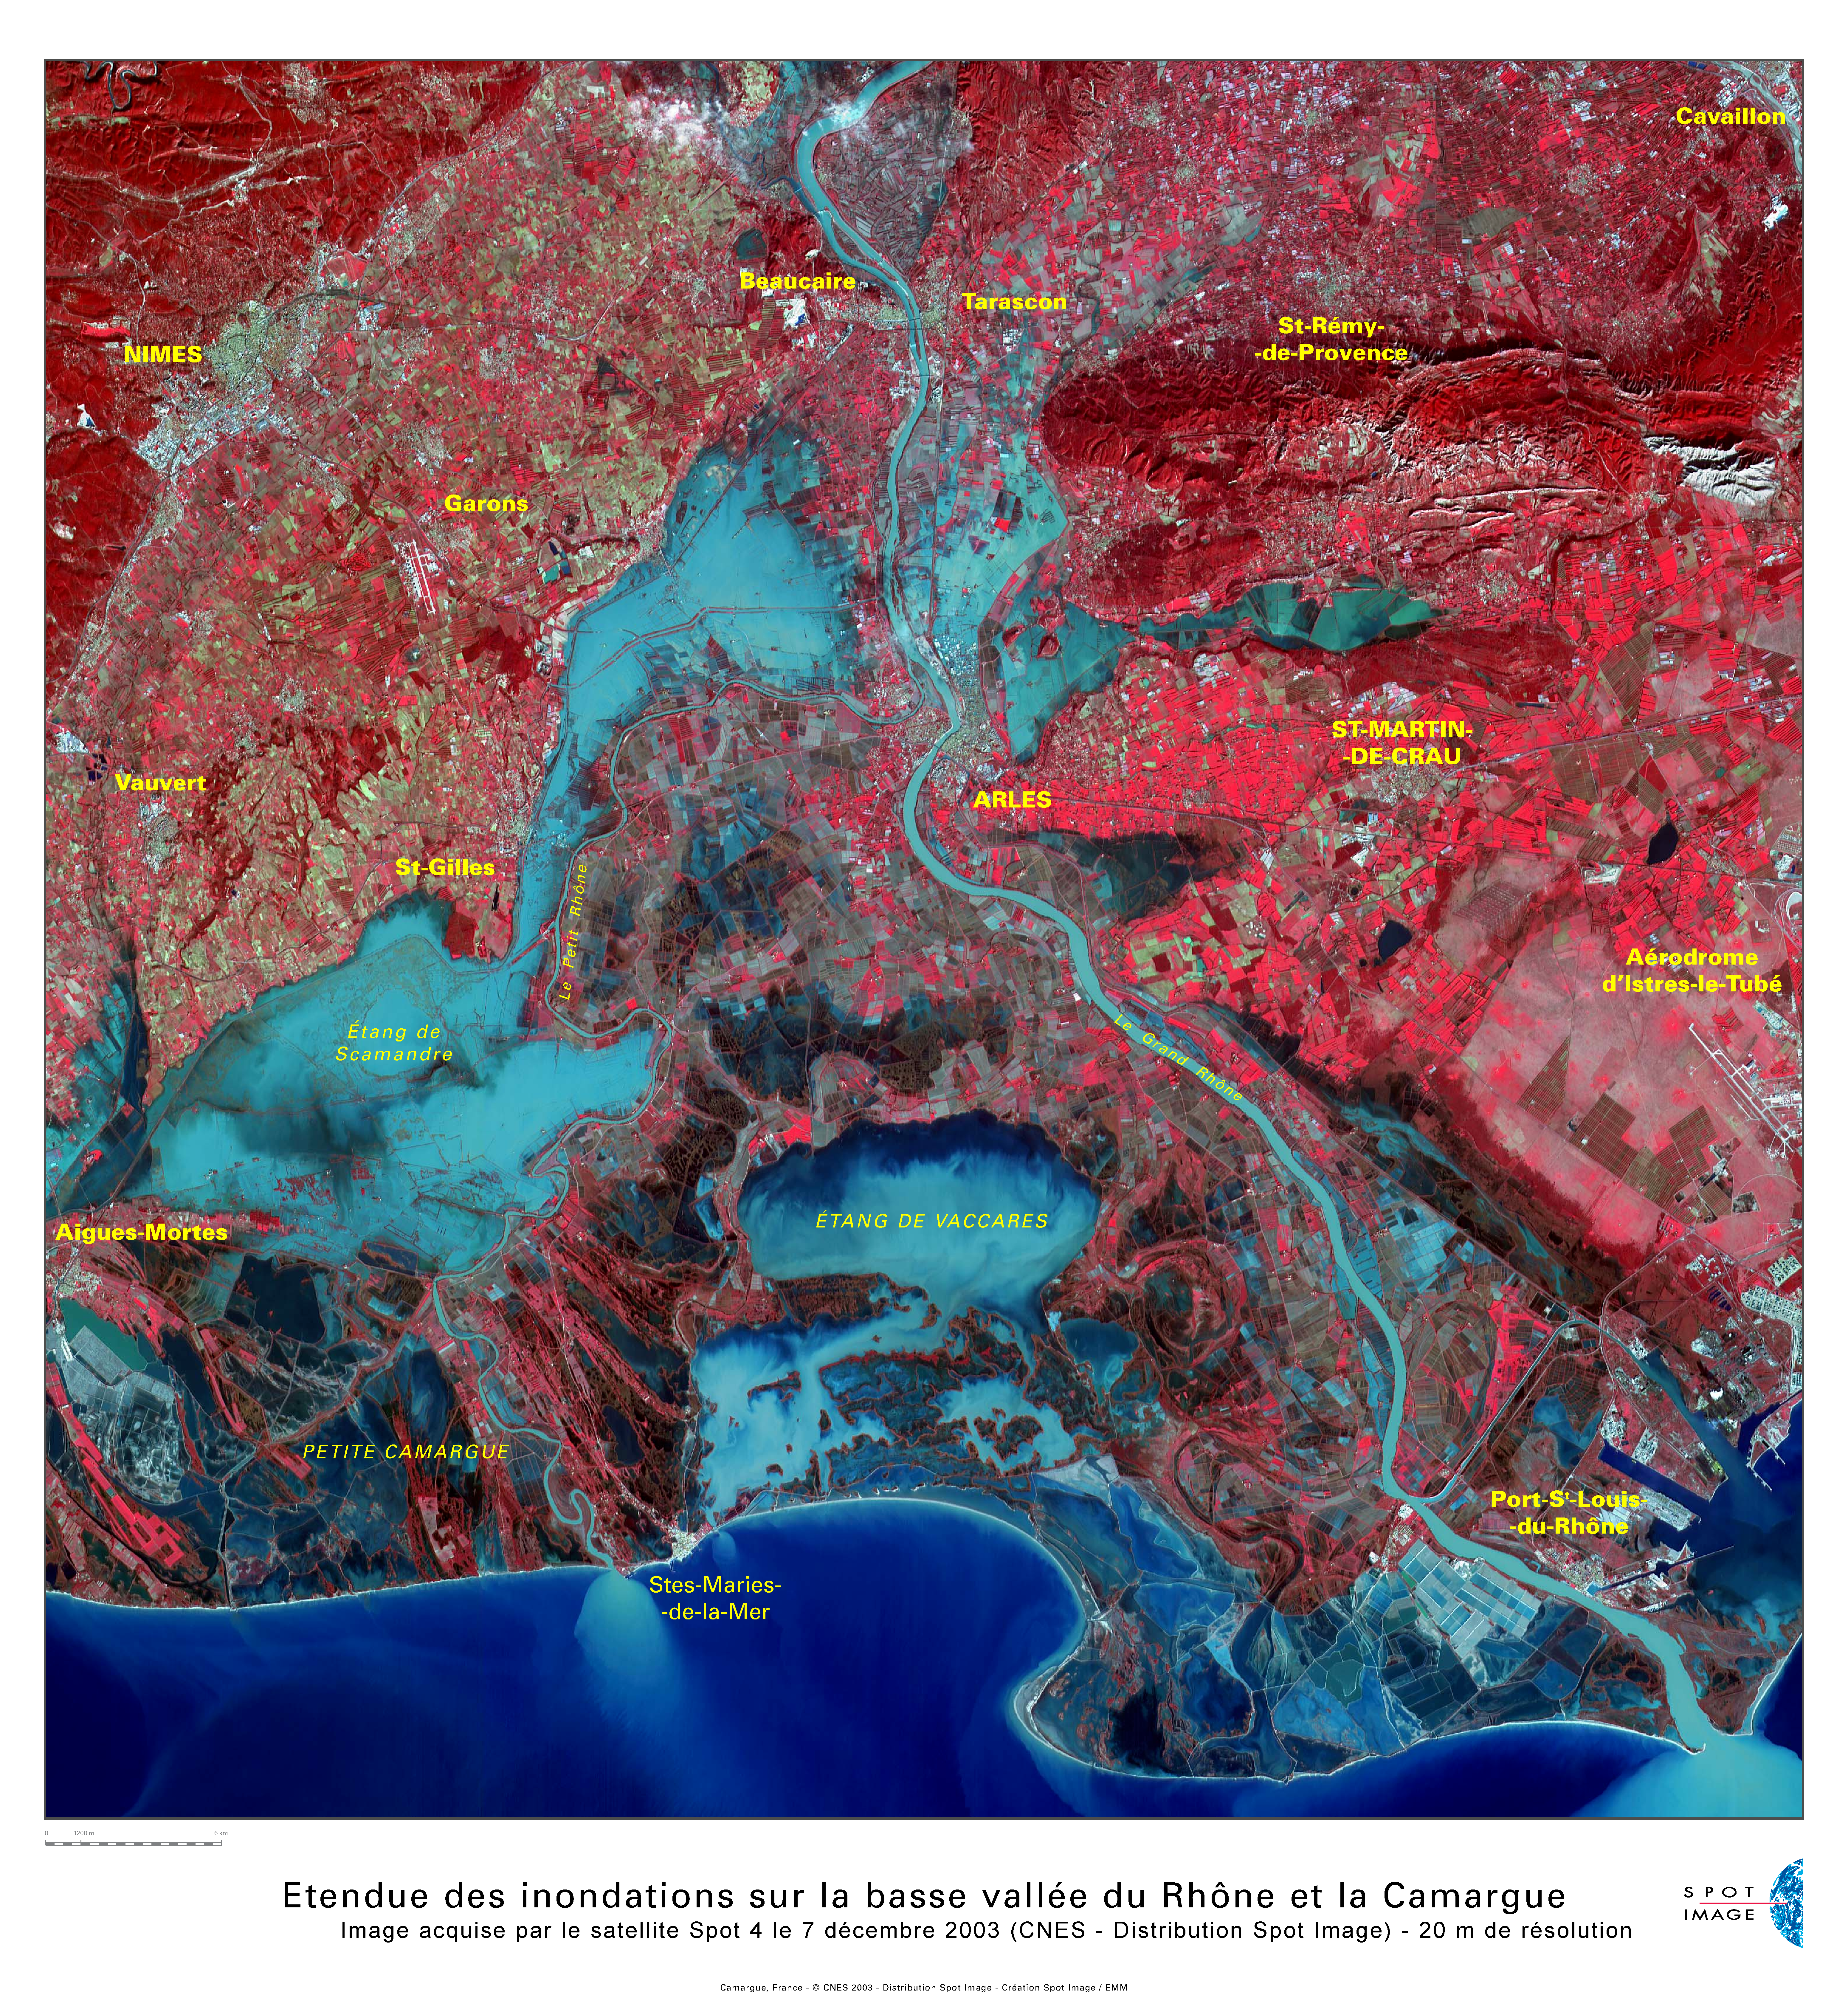
\includegraphics[width=.9\linewidth]{Chapitre1_Intro/Figures/SpotDec2003.pdf}	
	\caption{Image satellite de la basse vallée du Rhône le 7 décembre 2003, soit trois jour après la pointe de la crue. Les zones bleues représentent les cours d'eau ou les terres inondées, alors que les zones en rouge ou vert représentent des terrains secs. Source : CNES - Distribution Spot image.}
	\label{fig:Spot}
\end{figure}

\FloatBarrier
	\section*{Objectifs et organisation du manuscrit}
	\addcontentsline{toc}{section}{Objectifs et organisation du manuscrit}
%Là, tu peux citer les travaux qui ont cherché à dépasser ces limites, et indiquant tous les pbs qui restent non résolus. Et notamment l'utilisation de données historiques, LA piste prometteuse, mais en listant ce qui n'a pas été traité ou pas bien (incertitudes hydrométrie, méthodo intégrée de bout en bout, etc.).
%
%3/ expliquer ce que tu vas faire (objectifs et démarche scientifiques) : objectifs généraux, le site d'étude et pourquoi lui, l'organisation du manuscrit (il faut qu'on retrouve les grands points qui vont structurer les chapitres, et sur lesquels tu vas revenir en conclusion/perspectives).

	\paragraph{} La valorisation des données anciennes est l'un des moyens permettant d'améliorer les estimations des quantiles de crue extrêmes. La détermination et la propagation de l'ensemble des incertitudes lors de cet exercice est particulièrement importante mais elle est rarement effectuée. Un des objectifs de la thèse est de construire une méthode opérationnelle, complète et homogène, qui intègre les incertitudes à chaque étape de l'analyse fréquentielle afin de les propager jusqu'au résultat final. Dans ce contexte, l'utilisation de données historiques (pré-enregistrements continus) sera également explorée. L'utilisation de ces données est associée au concept de seuil de perception, qui est généralement supposé parfaitement connu dans la littérature. La prise en compte d'incertitudes affectant le seuil de perception et la durée de la période historique sera étudiée. La station hydrométrique du Rhône à Beaucaire constitue un cas d'étude idéal du fait de la longévité exceptionnelle des mesures de hauteur d'eau en continu (plus de deux siècles) et de l'immense patrimoine de données hydro-climatiques disponible dans la base de données HISTRHÔNE depuis le XIII \textsuperscript{ème} siècle. Les objectifs décrits ci-dessus seront étudiés dans ce manuscrit de thèse pour la station du Rhône à Beaucaire.
	
	\paragraph{} Ce manuscrit de thèse s'organise en trois parties dont les contours sont résumés dans la figure \ref{fig:SchemaThese}. Le premier chapitre permet de faire un bilan des données disponibles. Les relevés limnimétriques disponibles à Beaucaire depuis 1816  seront présentés en parallèle d'une étude de l'évolution des conditions d'écoulement de la zone au cours des deux derniers siècles. Les données de la base HISTRHÔNE jugées utiles à l'analyse fréquentielle des crues en seront extraites et des modèles hydrauliques seront utilisés pour tenter d'estimer le débit de ces événements anciens. 
	
	\paragraph{} Le second chapitre prend la forme d'un article scientifique soumis à "Journal of Hydrology" et accepté sous réserve de révision mineures. L'utilité des données limnimétriques historiques pour la réduction des incertitudes de l'analyse fréquentielle est explorée. La détermination et la propagation des différentes sources d'incertitude hydrométrique est effectuée pour la chronique du Rhône à Beaucaire de 1816 à 2020. On dispose alors d'une chronique continue de débits journaliers de plus de deux siècles. La part respective de l'incertitude hydrométrique et de l'incertitude d'échantillonnage au sein des estimations des quantiles de crue est ensuite examinée pour différentes tailles de chroniques. 
	
	\paragraph{} Le troisième chapitre reprend la série continue de débits de 1816 à 2020 estimée au chapitre précédent, ainsi que les données de la base HISTHRÔNE extraites au premier chapitre, afin de réaliser une analyse probabiliste des crues de 1500 à 2020. Le modèle probabiliste présenté dans ce chapitre permet de considérer les incertitudes de la chronique de débits continus (1816-2020), mais également la méconnaissance du seuil de perception et de la durée de la période historique. L'apport et les limites de l'utilisation des données historiques pour l'analyse fréquentielle des crues est explorée sous différentes hypothèses. 
	
	\paragraph{} Enfin une conclusion présente les principaux résultats et avancées obtenus pendant la thèse, puis des perspectives de travaux et études complémentaires.
	

\begin{figure}[h]
	\centering
	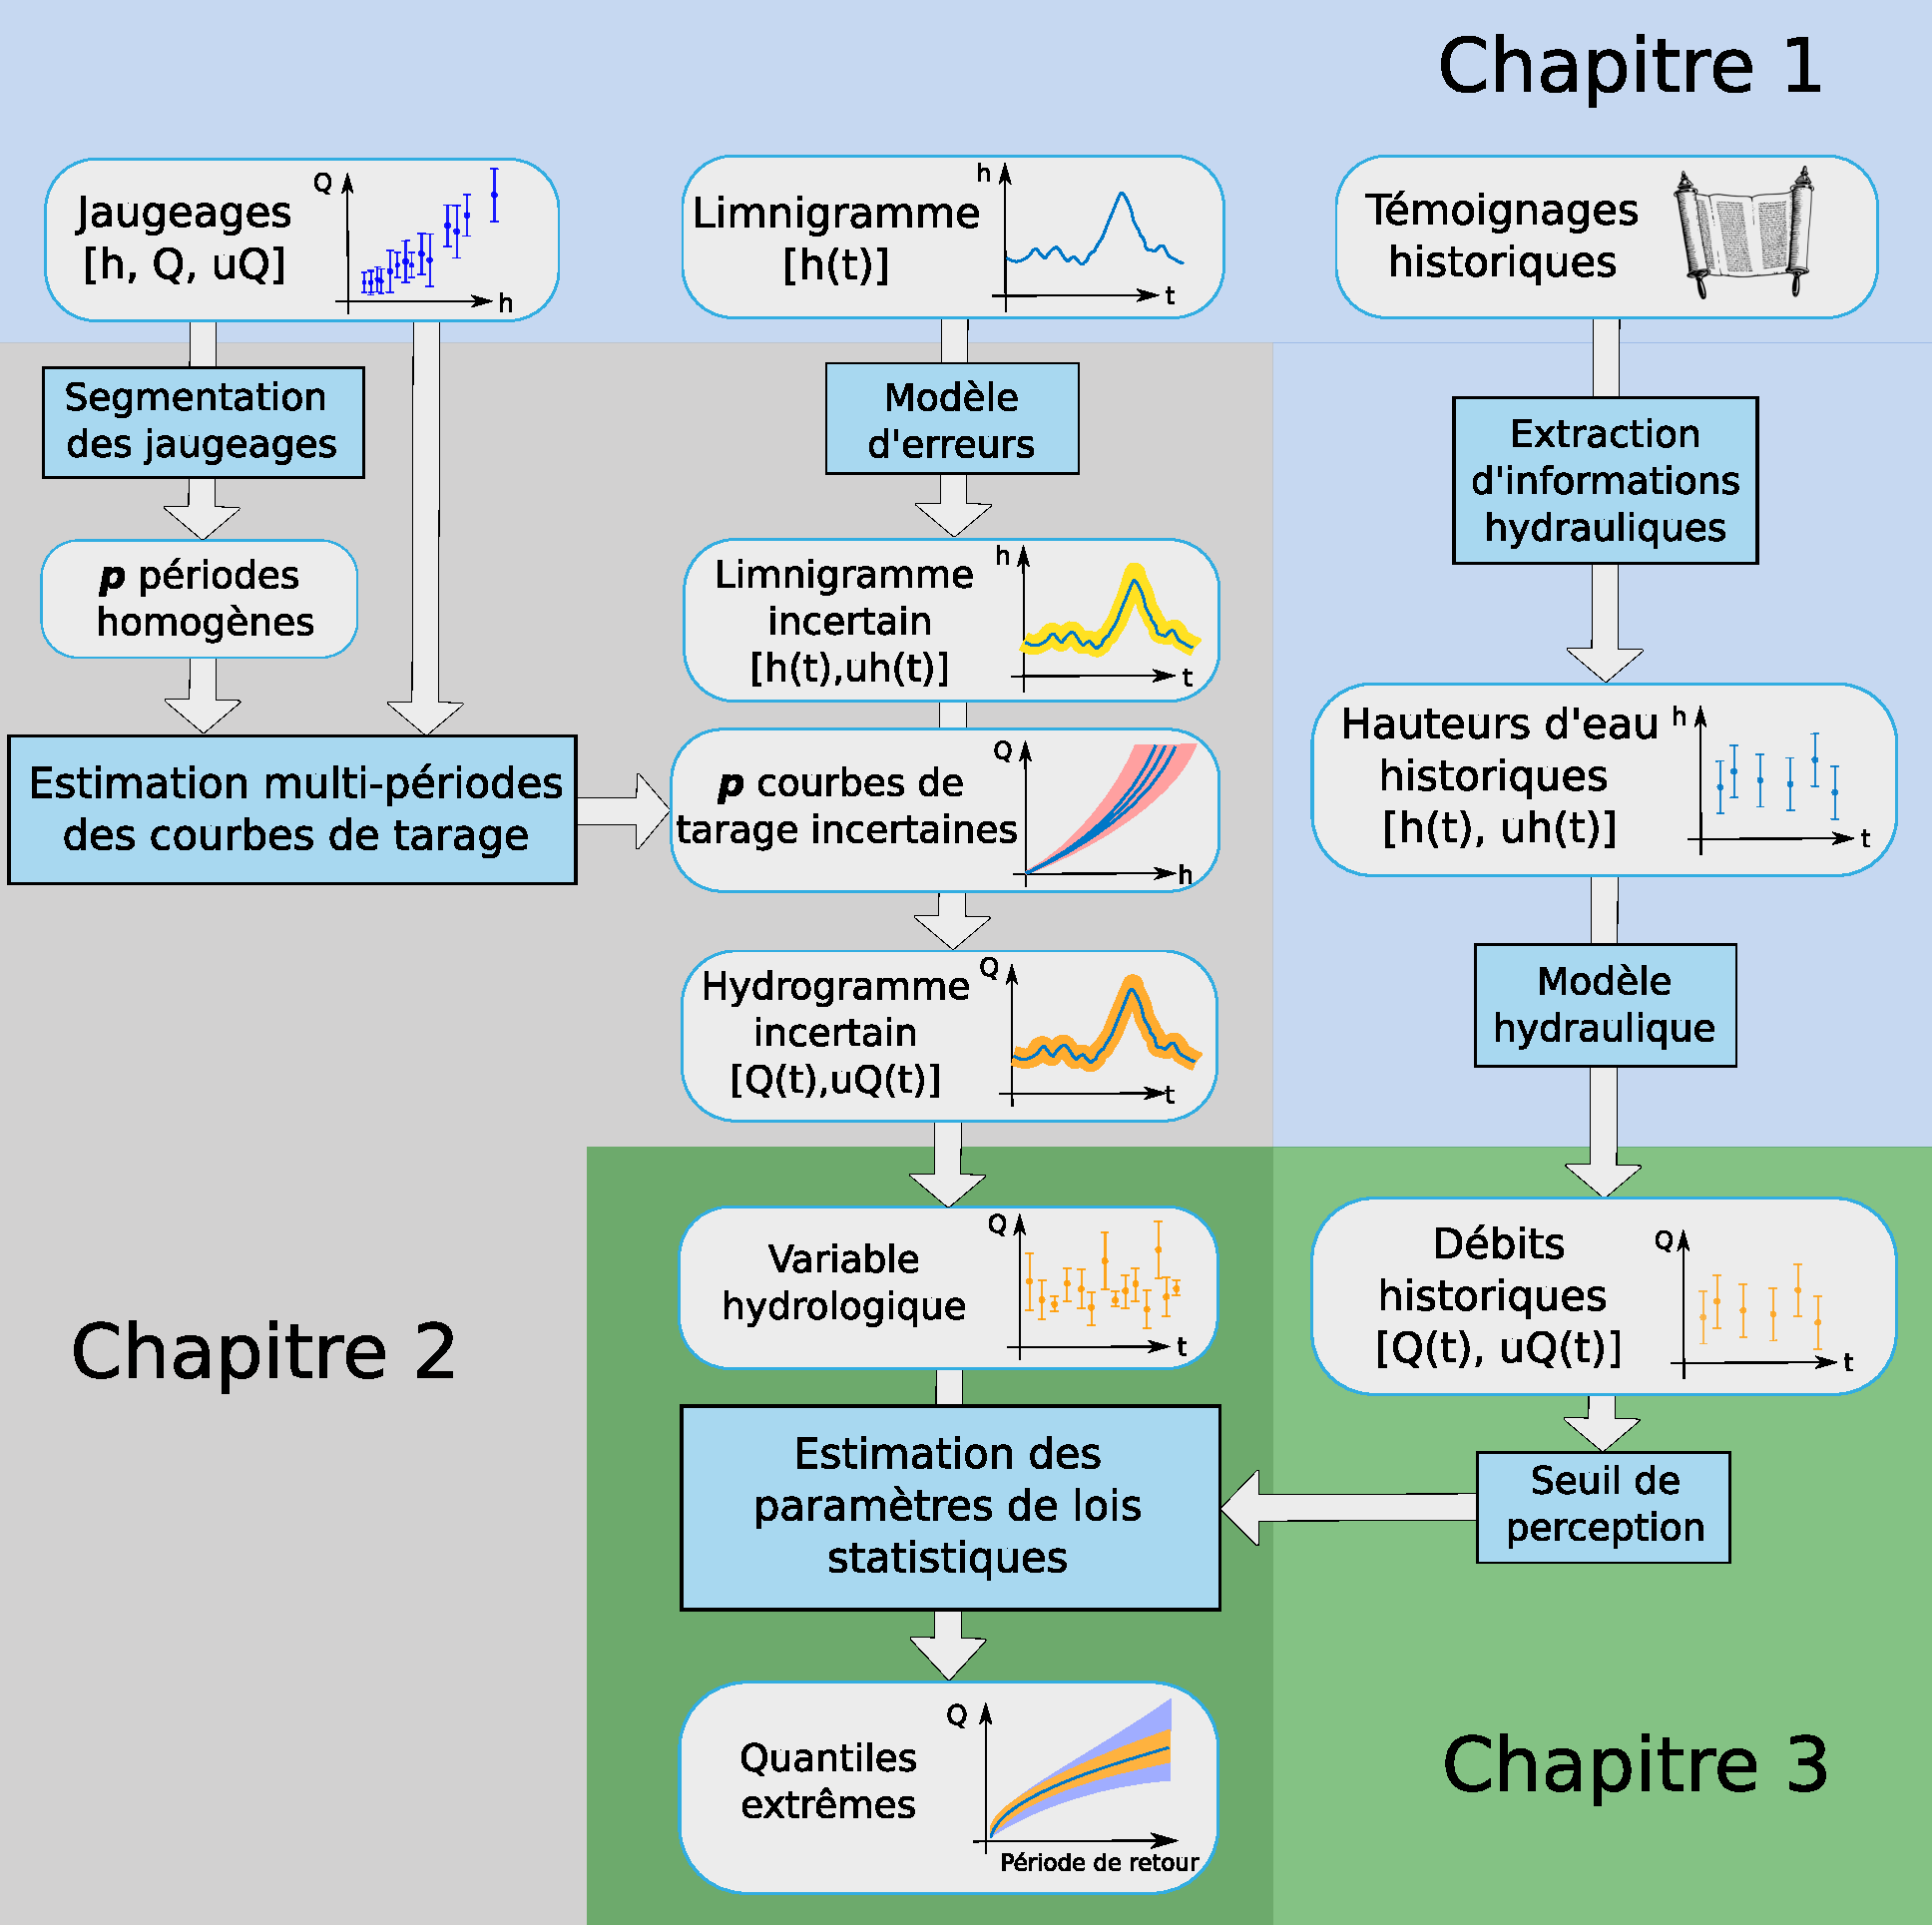
\includegraphics[width=.9\linewidth]{Chapitre1_Intro/Figures/SchemaThese.pdf}	
	\caption{Schéma d'organisation de la thèse. Les cases grises correspondent aux données et les cases bleues aux modèles et méthodes d'analyse. La lettre $h$ correspond à la hauteur d'eau, $Q$ au débit et $t$ au temps. La lettre $u$ correspond à l'incertitude qui affecte chacune de ces variables.}
	\label{fig:SchemaThese}
\end{figure}

\FloatBarrier

%\newpage
%%
%\printbibliography
%\end{document}
